\chapter{Theoretical Framework}

\section{Forces in Flight}

Fixed-wing aircraft are aerial vehicles whose flight depends on rigid aerodynamic surfaces (airfoils), unlike rotary-wing aircraft that rely on rotating blades to produce thrust and lift.

The fundamental principle of flight is governed by Newton's Second Law, which relates the net force acting on a body to its acceleration:

\begin{equation}
    \vec{F} = m\vec{a}
\end{equation}

where $\vec{F}$ is the resultant force vector, \textit{m} is the aircraft's mass, and $\vec{a}$ is the linear acceleration.

During flight, four main forces act on the aircraft: lift, weight, thrust, and drag. Lift is generated perpendicular to the airflow over the wings and results from a pressure difference between the upper and lower surface of the airfoil, explained by Bernoulli's principle and Newton's Third Law. According to Bernoulli's equation, the sum of static, dynamic pressure, and gravitational potential energy along a streamline is constant:

\begin{equation}
    p + \frac{1}{2} \rho v^2 + \rho g h = constant
\end{equation}

In many aerodynamic cases — like airflow over a wing — the altitude \textit{h}doesn’t change much, so the gravitational term can be neglected, giving the simplified form:

\begin{equation}
    p + \frac{1}{2} \rho v^2 = constant
\end{equation}

However the Bernoulli's principle are impractical for predicting lift in real-world scenarios due to factors like viscosity, turbulence, and three-dimensional flow effects. Therefore, an empirical approach using dimensionless coefficients is often employed. The lift force \textit{L} can be expressed as:

\begin{equation}
    L = C_L \frac{1}{2} \rho v^2 S
\end{equation}

where $C_L$ is the lift coefficient, \textit{$\rho$} is the air density, \textit{v} is the velocity of the aircraft relative to the air, and \textit{S} is the wing area. The lift coefficient $C_L$ is determined experimentally and depends on factors such as the angle of attack, airfoil shape, and Reynolds number.

Drag is the aerodynamic force that opposes the aircraft's motion through the air caused by friction and pressure differences. It can be expressed similarly to lift:

\begin{equation}
    D = C_D \frac{1}{2} \rho v^2 S
\end{equation}

where $C_D$ is the drag coefficient, which also depends on factors like shape, surface roughness, and flow conditions.

Thrust is generated by the aircraft's engines to overcome drag and propel the aircraft forward. The weight ($W = mg$) is the force due to gravity acting downward on the aircraft's mass.

\begin{figure}[H]
    \centering
    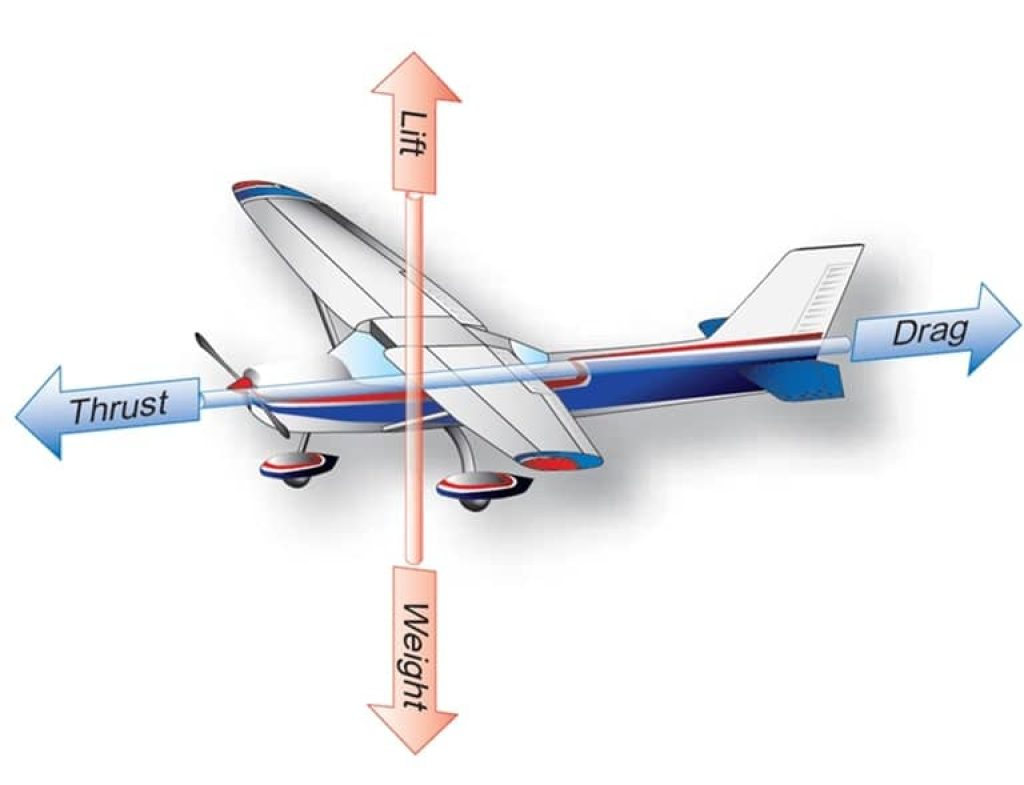
\includegraphics[width=0.8\textwidth]{figures/forces.jpg}
    \caption{Representation of lift and drag forces on a fixed-wing aircraft. \\ Source: StudyFlight (2025). Available at: \url{https://www.studyflight.com/understanding-the-aerodynamic-forces-in-flight/}. Accessed: Oct. 31, 2025.}
\end{figure}


The equilibrium of these forces determines the aircraft's flight conditions, such as steady level flight, climbing, or descending. Control surfaces like ailerons, elevators, and rudders manipulate these forces to change the aircraft's attitude and trajectory.

\section{Flight Dynamics and Control}


\section{Related Papers}